\documentclass[11pt,letterpaper]{article}
\usepackage{fullpage}
\usepackage{multicol}
\usepackage{amsmath}
\usepackage{amsfonts}
\usepackage{amssymb}
\usepackage{graphicx}
%\usepackage{pstricks, pst-node, pst-plot}

\newcommand{\ds}{\displaystyle}
\newcommand{\bv}{\mathbf}
\newcommand{\lv}{\langle}
\newcommand{\rv}{\rangle}

\begin{document}
\flushleft
\begin{multicols}{2}


\begin{large}\textbf{Math 115 Quiz 8: $\oint $ 4.3, 4.4 Optimization \\
Mon 15 November 2010}\end{large}

\textbf{Name:  }\underline{\hspace{35ex}}

\vspace{.5in}

\end{multicols}

\pagestyle{empty}

\flushleft

You have 30 minutes to complete this quiz.  Make your variables clear and
consistent (so if you want to say, for example, $\frac{dy}{dx}$, you should also
mention $y=f(x)$, or ``$y$ is a function of $x$'').  Calculators are OK.  

\begin{enumerate}
\item \textbf{Definitions/Concepts.} (1 pt each)
\begin{enumerate}
 \item Give an example of a family of functions, $f(x)$, depending on a parameter $a$, such that each member of the family has exactly one critical point.
\[f(x)=ax^2\]

\vspace{.5pc}
\item TRUE or \textbf{FALSE}: If the radius of a circle is increasing at a constant rate, then so is the area.

\vspace{.5pc}
The radius is a function of time, $r(t)$, hence so is the area $A(t)=\pi r(t)^2$.  Let $r'(t)=c$, the constant.  Then
\begin{eqnarray*}
 A'(t) &=& 2\pi r(t)\cdot r'(t) \\
&=& 2c\pi r(t) 
\end{eqnarray*}
is not constant, since $r$ is increasing.
\end{enumerate}

\vspace{1pc}
\item \textbf{Questions/Problems.}  Verify your extrema using either a well-labeled graph or the 2nd derivative.
\begin{enumerate}
 \item (2pts) What point(s) on the graph of $y=\frac{1}{x^2}$ is closest to
$(0,0)$?

\vspace{.5pc}
Let $R$ denote the square of the distance between the graph and the origin.  Then minimize $R$:
\begin{eqnarray*}
R &=& y^2+x^2 \\
&=& \left(\frac{1}{x^2}\right)^2+x^2 \\
 \frac{dR}{dx} =0 &=& \frac{-4}{x^5}+2x \\
&=& -4+2x^6 \\
2 &=& x^6 \\
\pm 2^{\frac{1}{6}} &=& x 
\end{eqnarray*}
Investigate the nature of the critical points:
\begin{eqnarray*}
 \frac{d^2R}{dx^2} &=& \frac{20}{x^6}+2 \\
&>& 0 \text{ for all }x
\end{eqnarray*}
so both are minima.  Therefore the points on the graph closest to the origin are $\left(\pm 2^{\frac{1}{6}}, 2^{-\frac{1}{3}})\right)\approx (\pm 1.122, 0.794)$.

\vspace{1pc}
\item (3 pts) I have a square piece of sheet metal, 1 meter on a
side. I plan to cut
equal squares from the four corners and fold up the
sides to make a box (with no
top). How big
should the cut-off squares be in order to maximize the
volume of the
box?  

\vspace{.5pc}
\begin{center}
 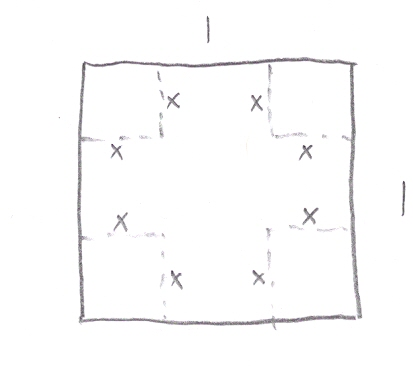
\includegraphics[scale=.2]{./q8solpic0001.jpg}
\end{center}

From the figure, the volume of the box is
\[V=x(1-2x)^2.\]
Maximize the volume:
\begin{eqnarray*}
 V &=& x(1-2x)^2 \\
&=& x-4x^2+4x^3 \\
\frac{dV}{dx} &=& 1-8x+12x^2=0
\end{eqnarray*}
The quadratic formula gives $x=\frac{8\pm \sqrt{4}}{24}$ so $x=\frac{1}{2},\frac{1}{6}$ are the critical points.
\[\frac{d^2V}{dx^2}=-8+24x\]
is positive when $x=\frac{1}{2}$ and negative when $x=\frac{1}{6}$ so the cutoff squares should be $\frac{1}{6}\times \frac{1}{6}\approx 1.167 \times 1.167$ m$^2$ (if the lengths were half a meter, then there would be no metal left).

\end{enumerate}

\vspace{1pc}
\begin{flushright}
 turn over $\rightarrow $
\end{flushright}

\pagebreak
\item \textbf{Computations/Algebra.} (1 pt each) Find the critical points.
\begin{enumerate}
\item $f(x)=(x-a)^2+b$
\begin{eqnarray*}
 f'(x)=0 &=& 2(x-a) \\
x &=& a 
\end{eqnarray*}

\vspace{.5pc}
\item $g(y)=y^3-ay^2+b$
\begin{eqnarray*}
 g'(y)=0 &=& 3y^2-2ay \\
&=& y(3y-2a) \\
y &=& 0,\frac{2a}{3} 
\end{eqnarray*}

\vspace{.5pc}
\item $h(z)=az(z-b)^2$
\begin{eqnarray*}
 h'(z)=0 &=& a(z-b)^2+2az(z-b) \\
&=& ((z-b)+2z)(z-b) \\
&=& (3z-b)(z-b) \\
z &=& \frac{b}{3},b 
\end{eqnarray*}

\vspace{1pc}
\end{enumerate}

\end{enumerate}
----------------------------------------------------------------------------------------

\vspace{1pc}
\noindent \textbf{ChAlLeNgE PrObLeM:}  Give an example of a function $f$ which satisfies the following.  If no such function exists, say why.  Assume $f''$ exists everywhere.  
\[f(x)f'(x)f''(x)f'''(x)<0 \text{ for all }x\]

\vspace{.5pc}
 \emph{(This problem was on the 1998 Putnam Mathematics Competition.  I took the solution from University of Hawaii's math department website.)}  

\vspace{.5pc}
No such exists.

\vspace{.5pc} 
\textit{Proof.  }By replacing $f(x)$ with $-f(x)$ if necessary, we can assume $f(x)>0$.  Similarly, by replacing $f(x)$ with $f(-x)$ if
necessary, we can assume $f'(x)> 0$.  Now to satisfy the condition $f''$ and $f'''$ must have different signs.  There are two cases:
\linebreak
Case 1: $f''(x)>0$ and $f'''(x)<0$.
\linebreak 
Since $f'''(x)< 0$, the graph of $f'(x)$ is concave down.  In particular, the graph of $f'(x)$ lies below its tangent line at $x=0$. Thus,
\[f'(x)\leq f'(0)+f''(0)x\]
and this implies
\begin{eqnarray*}
 f'\left(\frac{-f'(0)}{f''(0)}\right) &\leq & f'(0)+f''(0)\cdot \left(\frac{-f'(0)}{f''(0)}\right) \\
&=& 0
\end{eqnarray*}
contradicting $f'(x)$ is always positive.
\linebreak
Case 2: $f''(x)<0$ and $f'''(x)>0$.
\linebreak
Since $f''(x)<0$, the graph of $f(x)$ is concave down and hence the graph of
$f(x)$ lies below its tangent line at $x = 0$. Thus,
\[f(x)\leq f(0)+f'(0)x\]
and this implies
\begin{eqnarray*}
 f\left(\frac{-f(0)}{f'(0)}\right) &\leq & f(0)+f'(0)\cdot \left(\frac{-f(0)}{f'(0)}\right) \\
&=& 0
\end{eqnarray*}
contradicting $f(x)$ is always positive.

\begin{flushright}$\square $\end{flushright}

\end{document}


